The details of the numerical setup are presented in Section \ref{f1}.


least square smmothing (for pressure) discussed in \cite{hulb79}


\fbox{
\parbox{10cm}{{\bf features}
\begin{itemize}
\item $Q_1\times P_0$ element \index{$Q_1 \times P_0$}
\item incompressible flow \index{incompressible flow}
\item mixed formulation \index{mixed formulation}
\item isothermal \index{isothermal}
\item isoviscous \index{isoviscous}
\item analytical solution \index{analytical solution}
\end{itemize}
}}

\begin{center}
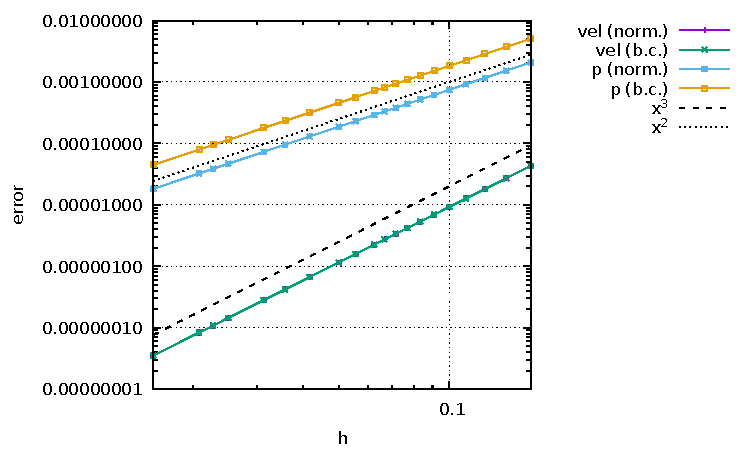
\includegraphics[width=6cm]{python_codes/fieldstone_saddlepoint_q1p0_nodalderivatives/errors}
\end{center}

\begin{center}
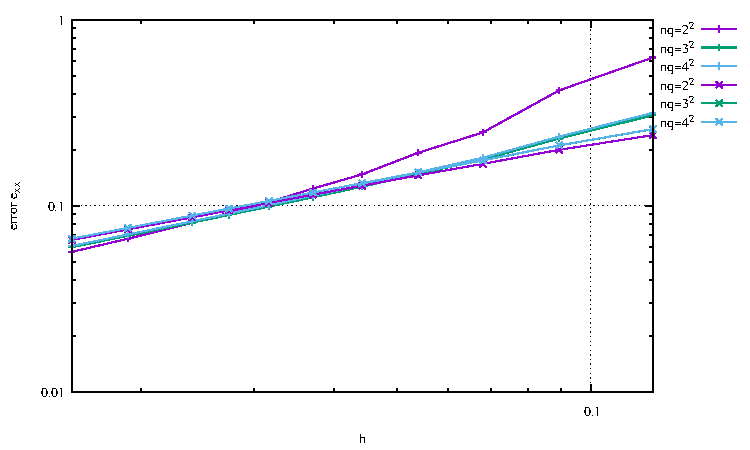
\includegraphics[width=6cm]{python_codes/fieldstone_saddlepoint_q1p0_nodalderivatives/errors_exx}
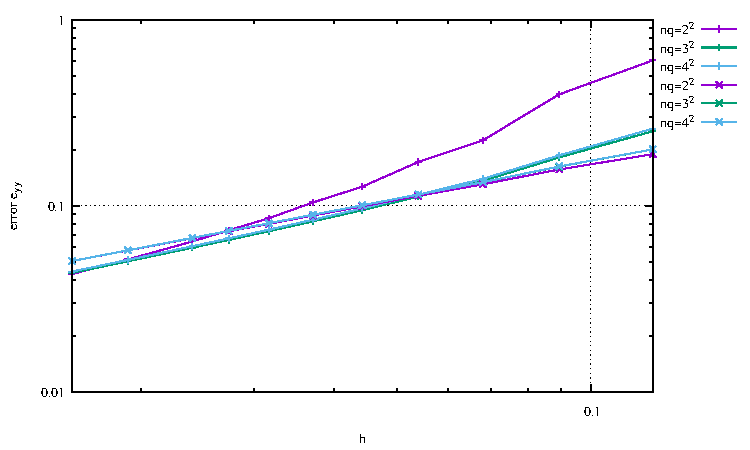
\includegraphics[width=6cm]{python_codes/fieldstone_saddlepoint_q1p0_nodalderivatives/errors_eyy}
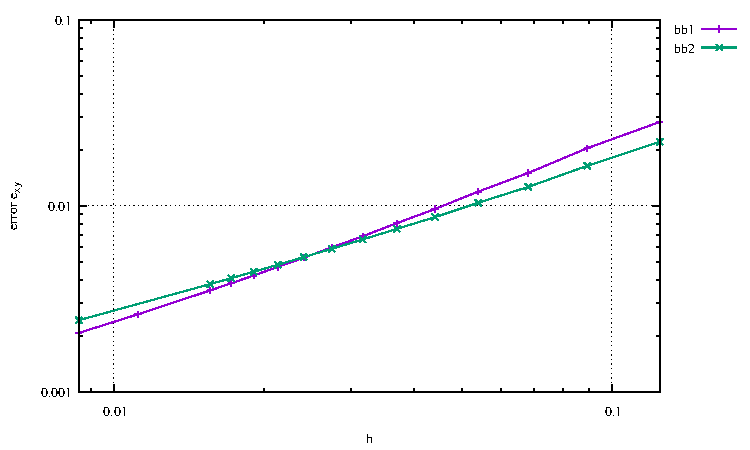
\includegraphics[width=6cm]{python_codes/fieldstone_saddlepoint_q1p0_nodalderivatives/errors_exy}
\end{center}
The error rate of convergence is quadratic for method 3 while it remains linear for methods 1 and 2!
